\documentclass[12pt, a4paper]{article}

\usepackage{booktabs}
\usepackage{graphicx}
\usepackage{hyperref}
\usepackage[margin=0.8in]{geometry} %set page margins
\usepackage{array} % needed for m column type in tabular
\usepackage[capitalise]{cleveref}

\usepackage{fancyhdr}
\pagestyle{fancy}
\setlength{\headheight}{28pt}

\fancyhead[L]{\myauthor}
\fancyhead[R]{\mydate}
\fancyhead[C]{\mytitle}

\fancyfoot[C]{\thepage}
\fancyfoot[L,R]{}
\renewcommand{\headrulewidth}{0.4pt}
\renewcommand{\footrulewidth}{0.4pt}

\newcommand{\mytitle}{Postcode Anonymity Analysis} %redefine these hear as they get wiped by \maketitle 
\newcommand{\mydate}{May 2021}
\newcommand{\myauthor}{Adam Hardy}
\title{\mytitle}
\author{\myauthor}
\date{\mydate}

\begin{document}
\maketitle

\section{Introduction}

In the US, 5-digit Zip codes are usually rounded to 3-digits when anonymising healthdata, so knowledge of the Zip code doesn’t allow small groups to be identified.  Even then, there are some 3-digit codes that have fewer than 20,000 residents, and the advice is to lump these together under a new code (000). Looking forward to how GDPR may affect data handling in the UK, is it possible to use a similar approach here?

UK postcodes can be in one of six formats and broken down into seven componenets that describe geographic areas (\cref{table:postcode_format}). Given how UK postcodes are constructed, we can`t simply truncate postcodes to three characters as is done for USA zip codes as this will result in postcode areas being combined together in ways which do not have real geographic meaning. For example, `NE3 1ED' and `NE35 2FG' are both valid postcodes. Truncating both of these to the first three characters would put these both in the `NE3' group. They should instead both be in an `NE' area group or separate `NE3' and `NE35' district groups (or another chosen postcode component group).

Below, we take a UK postcode population dataset\footnote{\url{http://www.nomisweb.co.uk/output/census/2011/Postcode_Estimates_Table_1.csv}} and perform an anonymity analysis of the postcode geographic components on the four population groups present in the dataset: total population, male population, female population and occupied households.

\begin{table}
\begin{center}
	\begin{tabular}{ m{0.125\textwidth}  m{0.1\textwidth}  m{0.1\textwidth}  m{0.07\textwidth}  m{0.1\textwidth}  m{0.1\textwidth}  m{0.1\textwidth}  m{0.07\textwidth}}
		Postcode Format & Outward Code & Inward Code & Area & District & Sub-District & Sector & Unit \\ \toprule
		AA9A 9AA & AA9A & 9AA & AA & AA9 & AA9A & AA9A 9 & AA \\
        A9A 9AA & A9A & 9AA & A & A9 & A9A & A9A 9 & AA \\
        A9 9AA & A9 & 9AA & A & A9 & \textbf{\textbf{N/A}} & A9 9 & AA \\
        A99 9AA & A99 & 9AA & A & A99 & \textbf{N/A} & A9 9 & AA \\
        AA9 9AA & AA9 & 9AA & AA & AA9 & \textbf{N/A} & AA9 9 & AA \\
        AA99 9AA & AA99 & 9AA  & AA & AA99 & \textbf{N/A} & AA99 9 & AA\\
	\end{tabular}
\end{center}
\caption{UK postcode formats and geographic components. `A` represents an alphabetic character, `9` represent a numeric character. Obtained from \url{https://ideal-postcodes.co.uk/guides/uk-postcode-format}.}\label{table:postcode_format}
\end{table}

\section{Anonymity Analysis}
\subsection{Postcode Component Selection}



We will use the area, district, sub-district and and sector. Where a postcode does not have a substrict, we will substitute the district in its place.



\begin{figure}
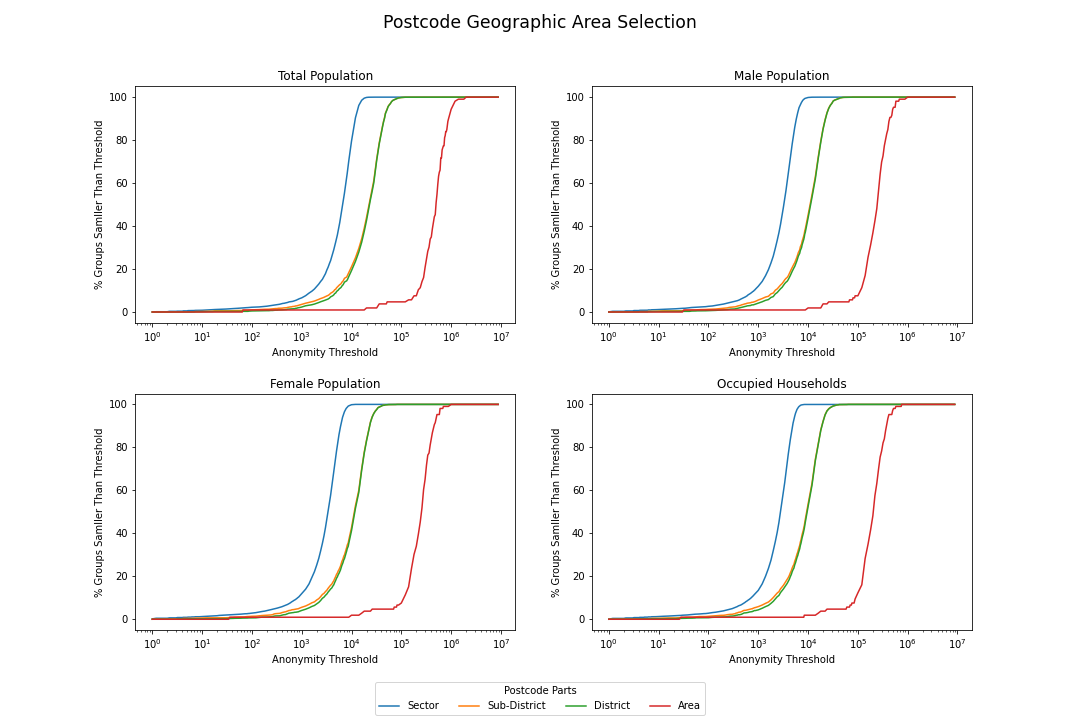
\includegraphics[width=1\textwidth,trim={0.1cm, 0.1cm, 0.1cm, 0.1cm},clip]{images/postode_selection.png}
\caption{postcode selection}\label{fig:postcode_selection}
\end{figure}

\subsection{Population Segment Selection}

\begin{figure}
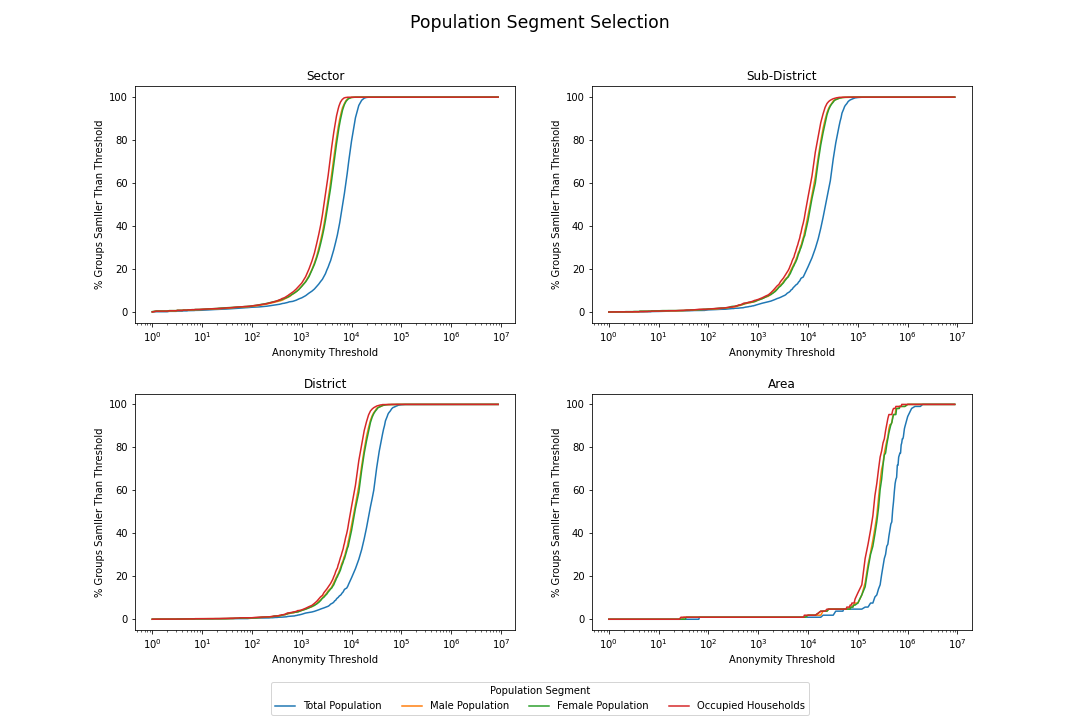
\includegraphics[width=1\textwidth,trim={0.1cm, 0.1cm, 0.1cm, 0.1cm},clip]{images/population_selection.png}
\caption{population selection}\label{fig:population_selection}
\end{figure}

\end{document}